\chapter{From Lines to Surfaces: A Preview of Local Approximation}

\section{A Bicycle Race in the Rain}

The Tour of Qinghai Lake reaches a downhill section as light rain begins. A helicopter camera looks down on a mountain road winding like a grey ribbon across green slopes. The commentator keeps repeating, ``The next bend is very sharp; the riders must slow down early.''

The riders do behave differently at different bends. At some, they barely touch the brakes and pass with a gentle lean. At others, they reduce speed well in advance and lean their bikes steeply, their tyres tracing arcs across the wet road. Clearly, sharp and gentle bends differ objectively; these are more than a commentator's flourishes.

Now imagine being the race engineer. The organizers hand you a plan of the route: a winding line on a map, with a scale but no contours or other information. They ask two apparently simple questions.

First: which bend is sharpest? Can you devise a ruler for measuring how much a road bends?

Second: why, when the map is enlarged many times, does every little piece of even a winding road look almost straight?

Before reading on, guess intuitively. For the first question, most people say that a bend is sharp when direction changes quickly. True, but that only rephrases the question: what does quickly mean, and in what units? The second question often gives people pause. It seems self-evident until someone asks why, and then it is not so obvious. These two questions begin our chapter.

\section{First Attempt: Some Unsuitable Rulers}

The simplest way to measure bending is to borrow a straight line. Curves are unfamiliar, but lines are old friends, so perhaps we can measure how far a bend departs from a line.

First ruler: join the bend's endpoints and measure the segment. A sharper bend should bring the endpoints closer and shorten the segment, right? Wrong. A long, gently curving arc and a short, abrupt hairpin can have exactly the same endpoint distance. That distance reflects how much of the road you selected, not how sharply it bends.

Second ruler: again join the endpoints, but measure the greatest distance from the curve to this chord, the so-called sagitta. Does greater height mean greater bending? Still no. Select a large piece of the same bend and the height may be large; select a small central piece and it shrinks. A measure that changes arbitrarily with the chosen interval cannot describe a degree of bending. That should be the bend's own property, not something an observer can alter at will.

Both failures suggest an important clue: bending must be determined near a point. You cannot judge it by standing far away and enclosing a large stretch; you must look close enough that even an arbitrarily small piece has a definite degree of bending. Mathematicians call this near-a-point viewpoint \textbf{local}. This chapter's central idea is that curved things are locally straight. To study bending, first find the line a curve locally resembles, then examine how it gradually departs from that line.

But what exactly does looking closely mean? How close is close? We need a clearer picture.

\section{Putting a Curve Under a Microscope}

Begin with something familiar that you may never have examined carefully: Earth is round, yet the playground under your feet looks flat. The playground is not special; you are small and Earth is large. Let us calculate. Walking an arc length $s$ on a circle of radius $R$ changes your direction by $s/R$ radians. Earth's radius is about $6\,400\,000$ metres, so walking $1$ metre along its surface changes direction by only
\[
\frac{1}{6\,400\,000}\ \text{radians} \approx 0.000\,008\,9^\circ.
\]
This angle is too small for any protractor to measure, so everyday experience insists that the ground is flat. Ancient people believed in a flat Earth because its local flatness is so convincing. Only sufficiently precise observations---comparing noon shadows at two places, or watching a distant ship's hull disappear before its mast---revealed the curvature behind that local appearance. Local flatness and global curvature are compatible: they are two faces of the same object at different scales.

Reverse the idea. Focus on a small piece of a winding curve and magnify it, then magnify again and again. Provided the curve is sufficiently smooth, without breaks or sharp corners, enough magnification makes it look straight. This happens with circles, parabolas, and maps of mountain roads. It is no coincidence; it expresses the meaning of smoothness. Under a microscope, a smooth curve is straight.

\begin{fanli}
``Every curve looks straight if magnified enough.'' False. Draw a V, the graph of $y=|x|$, and magnify its corner. Double it, enlarge it tenfold or a hundredfold: the same corner remains, with exactly the same angle. Magnification changes size, not angles. Looking locally straight is a privilege of smooth curves, unavailable to curves with corners or breaks. Mathematicians give this property a formal name, differentiability, which will be a main character in Part III. For now, remember that this chapter concerns smooth curves without sharp corners.
\end{fanli}

\begin{shiyan}
You can see magnification making a curve straight without special instruments. Draw a winding line and mark a fingernail-sized patch around one part with a pencil. Photocopy an enlargement centred on
the mark, then enlarge the copy again. After two or three rounds, the marked portion will look almost like a straight segment. A magnifying glass focused on a small portion gives a similar effect. Repeat with a sheet bearing a V and compare the corner: the counterexample is in your hands.
\end{shiyan}

\section{The Tangent: A Curve's Stand-in at a Point}

If a small piece of a smooth curve resembles a line, the next step is natural: find that line and make it the curve's stand-in near the point. Lines are familiar---a direction or slope can be described with one number. Translating a curved problem into a straight one immediately lowers the difficulty.

But which line is the best fit? A trap awaits. You might say that a tangent is a line touching the curve at only one point. That impression comes from circles and fails immediately for general curves. At the vertex of $y=x^2$, the vertical line also meets the parabola only once, but it is plainly the wrong stand-in: its direction does not follow the parabola at all. Conversely, a line fitting best locally may meet the curve again farther away. Meeting only once is a property of a circle's tangent, not the definition of a tangent.

The right idea grows from our failed rulers and repeated magnification. Fix a point $P$ on the curve, choose a nearby point $Q$, and join them by the line $PQ$. This is a \textbf{secant}; it cuts into the curve and describes the average direction from $P$ to $Q$. Now slide $Q$ along the curve toward $P$. The secant turns, its turning becomes smaller, and its position becomes more stable. The position it settles toward is the \textbf{tangent} at $P$.

\begin{center}
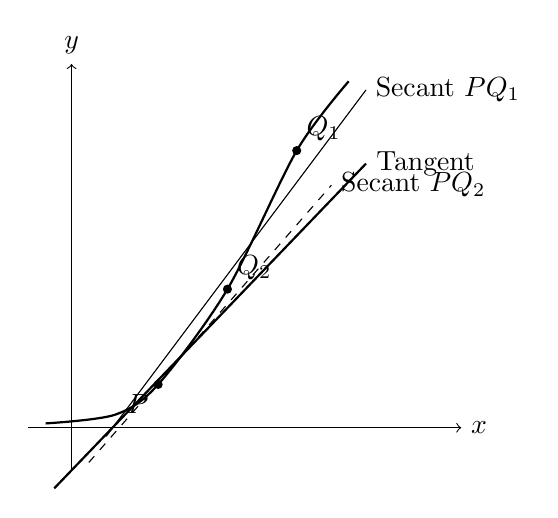
\begin{tikzpicture}[scale=1.1]
  \draw[->] (-0.5,0) -- (4.5,0) node[right] {$x$};
  \draw[->] (0,-0.5) -- (0,4.2) node[above] {$y$};
  \draw[thick] plot[smooth] coordinates {(-0.3,0.05) (0.5,0.15) (1,0.5) (1.8,1.6) (2.6,3.2) (3.2,4.0)};
  \fill (1,0.5) circle (1.5pt) node[below left] {$P$};
  \fill (2.6,3.2) circle (1.5pt) node[above right] {$Q_1$};
  \fill (1.8,1.6) circle (1.5pt) node[above right] {$Q_2$};
  \draw (0.4,-0.1) -- (3.4,3.9) node[right] {Secant $PQ_1$};
  \draw[dashed] (0.2,-0.4) -- (3.0,2.8) node[right] {Secant $PQ_2$};
  \draw[thick] (-0.2,-0.7) -- (3.4,3.05) node[right] {Tangent};
\end{tikzpicture}
\end{center}

\begin{dingyi}[An Intuitive Definition of the Tangent]
Let $P$ lie on a smooth curve, and choose another point $Q$ on it. The definite line approached by the secant $PQ$ as $Q$ moves arbitrarily close to $P$ along the curve is called the tangent at $P$.
\end{dingyi}

A subtle point hides in this definition: $Q$ can never actually equal $P$. Two points determine a line; once $Q$ reaches $P$, the secant ceases to exist. A tangent is determined by a process that never reaches its endpoint. For now we accept it intuitively. The difficulties it creates, and how mathematicians tame it into a rigorous limit, belong to the next chapter.

\begin{shuyu}{Tangent}
Intuition: a curve's best straight-line stand-in at a point, the shape seen under a microscope. Formal definition: the limiting position of the secant $PQ$ as $Q$ approaches $P$. Example: at every point of a circle, the tangent is perpendicular to the radius through that point.
\end{shuyu}

That example deserves scrutiny because it checks the new idea against old knowledge. Elementary geometry says that a circle's tangent is perpendicular to its radius. Can approaching secants recover this? Yes. Let the centre be $O$, choose $P$ on the circle, then choose $Q$ and $Q'$ symmetric about $OP$. Symmetry makes the chord $QQ'$ perpendicular to $OP$. Slide $Q$ and $Q'$ simultaneously toward $P$ around the circle. They remain symmetric at every step, so the secant remains perpendicular to $OP$. Its limiting position, the tangent, is therefore perpendicular to $OP$ too. The new method makes the old conclusion a special case of a wider picture. That is an important test of a mathematical idea's reliability.

What use is this stand-in? Plenty. If a wheel suddenly loses its grip while turning, the vehicle shoots off in the tangent direction. A hammer thrower's hammer flies tangentially when released, and sparks from a grinding wheel do the same. A curve's intention at each instant is written in its tangent.

\section{How Sharply Does It Bend? Curvature}

With tangents, direction becomes precise: a curve's direction at a point is its tangent's direction. We can now build our ruler for bending.

Imagine being an ant crawling along a curve with a compass continuously recording the angle of your direction. Over equal distances, the compass barely moves on a gentle stretch but turns rapidly at a sharp bend. We can therefore define the degree of bending as how much direction changes per unit arc length.

\begin{dingyi}[A Preliminary Definition of Curvature]
The curvature at a point of a smooth curve is the rate at which the tangent's direction angle changes with arc length: near that point, the number of radians the tangent turns per unit arc length travelled. Greater curvature means sharper bending.
\end{dingyi}

The definition is somewhat abstract, but one family of curves lets us calculate it completely: circles.

\begin{dingli}[The Curvature of a Circle]
A circle of radius $R$ has the same curvature everywhere, equal to $\dfrac{1}{R}$.
\end{dingli}

\begin{proof}
Start at a point on the circumference and travel an arc length $s$ to another point. Let the corresponding central angle be $\theta$, measured in radians. The arc-length formula gives
\[
s = R\theta.
\]
Now consider the change in direction. The radius is always perpendicular to the tangent. From start to finish, the radius turns through the central angle $\theta$. Perpendicularity is preserved during this turning, so the tangent also turns through $\theta$. Thus the ratio of direction change to arc length is
\[
\frac{\theta}{s} = \frac{\theta}{R\theta} = \frac{1}{R}.
\]
This ratio contains no information about the starting point, so it is the same everywhere on the circle, as required.
\end{proof}

\begin{li}
On a roundabout of radius $10$ metres, every $1$ metre travelled changes direction by $\dfrac{1}{10}$ radian, about $5.7^\circ$. On a sharp bend of radius $2$ metres, every $1$ metre changes direction by $\dfrac{1}{2}$ radian, about $28.6^\circ$. The latter has five times the curvature. Sharper bending means smaller radius and greater curvature, matching our intuition.
\end{li}

\begin{center}
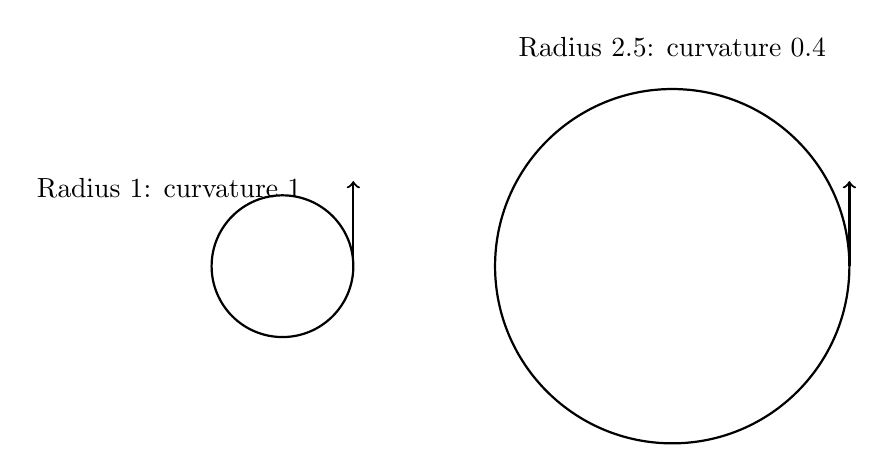
\begin{tikzpicture}[scale=0.9]
  \draw[thick] (0,0) circle (1);
  \draw[->,thick] (1,0) -- (1,1.2);
  \node at (-1.6,1.1) {Radius $1$: curvature $1$};
  \draw[thick] (5.5,0) circle (2.5);
  \draw[->,thick] (8,0) -- (8,1.2);
  \node at (5.5,3.1) {Radius $2.5$: curvature $0.4$};
\end{tikzpicture}
\end{center}

\begin{zhu}
A straight line never turns, so its direction angle is constant and its curvature is $0$. Through the formula $\dfrac{1}{R}$, we can regard it as a circle of infinite radius. This is a useful viewpoint: a line is a curve with zero bending, as naturally as $0$ represents none.
\end{zhu}

\begin{shuyu}{Curvature}
Intuition: how sharply something bends, measured by the turn in direction per unit distance. Formal definition: the rate of change of the tangent's direction angle with arc length; a circle's curvature is the reciprocal of its radius. Example: a circle of radius $4$ centimetres has curvature $\dfrac{1}{4}$ radian per centimetre.
\end{shuyu}

Curvature is part of engineers' everyday work. A railway joining a straight track to a bend must not let curvature jump abruptly from $0$ to $\dfrac{1}{R}$, or the train suffers a violent sideways jolt. A clever design inserts a transition in which curvature rises smoothly and gradually from zero to $\dfrac{1}{R}$, almost unnoticed by passengers. Motorway ramps, roller-coaster tracks, and the tightening arcs at loop entrances all use the same principle: let the amount of bending change smoothly. An abstract definition of direction change per unit arc length ends up helping every passenger's seat belt.

A general curve has different curvatures at different places: mountain-road straights have curvature $0$, gentle bends little curvature, and sharp bends much. Mathematicians use a natural and elegant approach: at each point find the circle that fits the curve best, neither too loose nor too tight. This is the \textbf{osculating circle}, and the point's curvature is the reciprocal of its radius. At a straight portion that radius is infinite; at a sharp bend it is small and tight. For now this is only an intuitive description. A rigorous definition needs derivatives and must wait for the next part. But notice our method: approximate a curve by a line, then approximate its departure from the line by a circle. Step by step, bending becomes increasingly precise local approximation, a path leading deep into differential geometry.

\section{Another Perspective: Straight Lines on a Sphere}

So far we have stayed in the plane. Change the stage and see how far these ideas travel.

Open a flight-tracking app and examine a flight from Beijing to New York. On an ordinary flat map, its route is not straight but a broad northward arc passing near the Arctic Circle. Why the detour? There is no detour. Flattening a sphere into a map distorts shapes; on the real sphere, this curved-looking route is almost the straightest path.

In the plane, straight and shortest describe two sides of the same property: a segment is the shortest connection between two points. Carry that property to a sphere to identify its straight lines, the shortest routes between two surface points. They follow circles cut by planes through the sphere's centre: \textbf{great circles}. The equator and every complete meridian circle are great circles. Other latitude circles are not, since their planes miss the centre, so following a latitude is not the shortest route.

\begin{shuyu}{Great Circle}
Intuition: a straight line on a sphere, giving its straightest and shortest routes. Formal definition: a circle formed by intersecting a sphere with a plane through its centre, also called a geodesic. Example: the equator and every complete meridian circle are great circles; a short route from Beijing to New York follows one.
\end{shuyu}

Something astonishing happens once great circles appear. Use their arcs as sides on a sphere and you can form spherical triangles. Consider one explicitly: start at the North Pole, follow a meridian south to the equator, travel east along one quarter of the equator, then follow another meridian north to the pole. All three sides are great-circle arcs, forming a standard spherical triangle. What is its interior angle sum?

\begin{dingli}[A Triangle with Three Right Angles]
The spherical triangle just described has three angles of $90^\circ$, summing to $270^\circ$.
\end{dingli}

\begin{proof}
There are two steps. First, examine the equatorial angles. At each intersection, the equator points east and the meridian north. East--west and north--south are perpendicular, so each meridian meets the equator at $90^\circ$: both base angles are right. Second, examine the polar angle. The angle between the meridians at the pole equals their longitude difference. Travelling one quarter of the equator gives exactly $360^\circ \div 4 = 90^\circ$ of longitude difference. All three angles are $90^\circ$, summing to $270^\circ$.
\end{proof}

\begin{center}
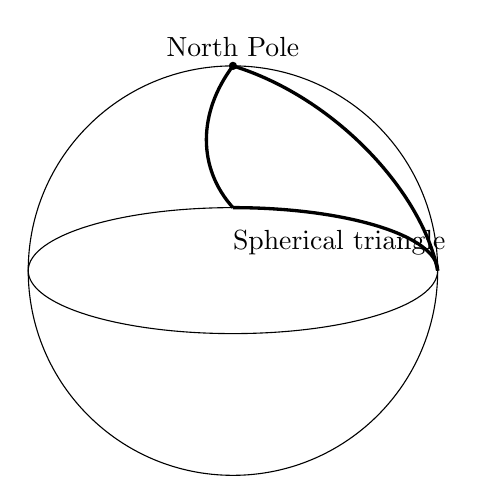
\begin{tikzpicture}[scale=1.0]
  \draw (0,0) circle (2.6);
  \draw (0,0) ellipse (2.6 and 0.8);
  \draw[very thick] (0,2.6) .. controls (1.3,2.2) and (2.4,1.0) .. (2.6,0);
  \draw[very thick] (0,2.6) .. controls (-0.45,2.0) and (-0.45,1.3) .. (0,0.8);
  \draw[very thick] (2.6,0) arc[start angle=0, end angle=90, x radius=2.6, y radius=0.8];
  \fill (0,2.6) circle (1.5pt) node[above] {North Pole};
  \node at (1.35,0.35) {Spherical triangle};
\end{tikzpicture}
\end{center}

$270^\circ$! One of plane geometry's firmest laws says triangle angles always sum to $180^\circ$. On a sphere it fails, with a whole extra $90^\circ$. That extra amount is called the \textbf{spherical excess}. First see how large the triangle is. The two meridian circles divide the sphere from pole to pole into four wedges, and the equator halves each into north and south. Our triangle is one piece, or one-eighth of the sphere. Larger triangles have greater excess: this one-eighth-sphere triangle has $90^\circ$ excess. Walk only one-eighth of the equator before returning, and the triangle shrinks, its polar angle becomes $45^\circ$, its angle sum $225^\circ$, and its excess halves. In the early nineteenth century, mathematicians distilled this observation into an exact theorem: a spherical triangle's excess is proportional to its area. On a sphere of radius $R$, the excess in radians equals the area divided by $R^2$. We will not give the full proof, but the intuition is clear: a larger triangle encloses more curvature, while a tiny one nearly lies in a plane and its angle sum nearly returns to $180^\circ$.

Pause to appreciate that last point. An ant living on a sphere need not fly into space to see its world's curvature. It can draw a triangle on the ground and measure its angle sum. Curvature is written into the surface's own geometrical laws and can be detected with rulers, protractors, and light. Mathematicians call this an \textbf{intrinsic} property. Both the ground beneath us and the heavens above can be investigated from within in this way.

\begin{lianjie}
This chapter's ideas have relatives throughout the book and beyond it. Looking ahead, the limiting process in secants approaching a tangent is Chapter 9's main character; tangent slope is the geometrical face of the derivative in Chapter 10; and curvature and spherical geometry grow into differential geometry in Chapter 17. Beyond the book, satellite navigation uses great circles rather than straight map lines for surface distances. Einstein's general relativity goes further: gravity is the curvature of spacetime, and planets orbit the Sun along straight lines in that curved spacetime. Even our ant has real counterparts: surveyors measure triangle angle sums on the ground to investigate Earth's surface shape.
\end{lianjie}

\begin{shiyan}
Find an orange, apple, or tennis ball, a marker, and a flexible tape measure. Draw an equator around its middle and two meridians through its poles, meeting at roughly a right angle. Their arcs enclose a spherical triangle. Tear a small paper wedge as an angle template, or hold a protractor against the surface to estimate the three angles. Each is near $90^\circ$, and the sum clearly exceeds $180^\circ$. Finally, try something more destructive: peel the orange and flatten a piece of peel on a table. It must either curl upward or split. A spherical surface cannot flatten without stretching or tearing. This is why every world map must distort something, and it is tangible evidence of curvature.
\end{shiyan}

\begin{toolbox}
This chapter adds five tools to your backpack.
\begin{itemize}
  \item \textbf{Local approximation through magnification}: study bending by enlarging a small piece. Smooth curves locally resemble lines; smooth surfaces locally resemble planes.
  \item \textbf{From secants to tangents}: average direction approaches instantaneous direction. A tangent is the limiting secant, a curve's straight-line stand-in at a point.
  \item \textbf{Curvature}: direction change per unit arc length measures bending. A circle has curvature $= 1/R$, and a line has curvature $0$.
  \item \textbf{Great circles and geodesics}: the straightest surface routes are defined through shortest paths; on a sphere they follow circles cut by planes through its centre.
  \item \textbf{Spherical excess}: the amount by which a spherical triangle's angle sum exceeds $180^\circ$, proportional to area. It makes curvature measurable from within the surface.
\end{itemize}
\end{toolbox}

\begin{pandeng}
For further climbing, remember these terms for later encounters in school, university, or competition reading: limits and derivatives, making arbitrarily close rigorous; osculating circles and radii of curvature, second-order local approximations of curves; Gaussian curvature and Gauss's remarkable theorem, showing that surface curvature is determined entirely by measurements within the surface; geodesics and Riemannian geometry; and popular accounts of curved spacetime in general relativity. Behind each term stands an intuitive picture already met here.
\end{pandeng}

\section*{Questions to Think About}

\textbf{Observation}

\begin{sikao}
  \item Find a familiar bend, such as your route to school, a track at the playground, or a roller-coaster diagram. Mark where you think curvature is greatest and least. Hint: imagine driving along it. Where must the steering wheel turn most sharply, and where hardly at all?
  \item On a globe, examine the equator, meridian circles, and the latitude circle at $60^\circ$ north. Which are great circles? Is flying due east from Beijing along $60^\circ$ north to a European city at the same latitude the shortest route? Hint: imagine slicing Earth with a plane through its centre. Does the plane of that latitude circle pass through the centre?
\end{sikao}

\textbf{Proof}

\begin{sikao}
  \item Verify a circle's curvature using an entire semicircle instead of the arc-length formula $s=R\theta$. Travelling halfway around, how much does the tangent direction turn, and how far do you travel? Does their ratio still give $\dfrac{1}{R}$? Hint: the tangent directions at the semicircle's endpoints are opposite, and the arc length is $\pi R$.
  \item Prove that the three-right-angle spherical triangle occupies exactly one-eighth of the sphere, and verify that its excess in radians equals its area divided by $R^2$. Hint: the whole sphere has area $4\pi R^2$. Is one-eighth of the sphere made of four such triangles or eight? The excess is $270^\circ - 180^\circ$; remember to convert degrees to radians.
\end{sikao}

\textbf{Challenge}

\begin{sikao}
  \item Roll a rectangular sheet into a cylinder without stretching or tearing it. What happens to a straight segment drawn on the paper? Do triangle angles on the cylinder sum to more than $180^\circ$? Hint: without stretching or tearing, every length and angle on the sheet is preserved. Could an ant living there distinguish a plane from a cylinder using our angle-sum method? How does this differ fundamentally from a sphere?
  \item An ant carries a small arrow around a spherical triangle, keeping it as far as possible pointing forward without spinning along each edge, then changing direction with the triangle's corners. After one circuit, does the arrow point as it did initially? If not, by how much does it differ? Hint: try the plane first, where the answer should be unchanged, then the spherical right triangle. Add the corner turns and compare with spherical excess.
\end{sikao}

\section*{The Door to the Next Chapter}

Looking back, we have essentially invited the infinitely small into mathematics. Magnified indefinitely, a smooth curve resembles a line; a tangent is where secants go as $Q$ approaches $P$ without bound; curvature is the rate of direction change on an infinitesimal piece; and sufficiently small spherical triangles have angle sums arbitrarily close to $180^\circ$. Every central concept rests on a process of endless approach without arrival.

Today we accepted all of this through intuition. But when $Q$ slides toward $P$, how close is close enough? What distinguishes approaching indefinitely from arriving? If a theory's foundations use such vague verbs, why trust its conclusions?

More than two hundred years ago, mathematicians wrestled with these same questions and argued for over a century before finding an answer: the \textbf{limit}. It translates endless approach into precise, testable inequalities. Limits form the foundation of Part III and the starting point for derivatives, integrals, and the mathematics of change. Next chapter we confront the spectre behind every smooth curve and bend: is the infinitesimal a legitimate mathematical object?
